\documentclass[tikz, border=2pt]{standalone}

\usepackage{amsmath,amssymb}
\usepackage{pgfplots}
\pgfplotsset{compat=1.18}
\usetikzlibrary{arrows.meta}
\usepackage{xcolor}

\definecolor{utnblue}{RGB}{0, 51, 102}

\begin{document}
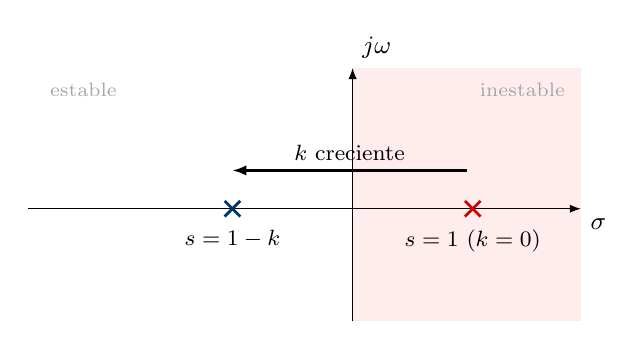
\begin{tikzpicture}[>=Latex, font=\small]
\begin{axis}[
    axis lines=middle,
    axis on top,
    axis line style={-{Latex[length=4pt]}},
    width=8.6cm, height=4.8cm,
    xmin=-2.7, xmax=1.9,
    ymin=-1.0, ymax=1.25,
    xlabel={$\sigma$}, ylabel={$j\omega$},
    xlabel style={anchor=north west},
    ylabel style={anchor=south west},
    xtick=\empty, ytick=\empty,
    clip=false,
]
    % semiplano derecho: region inestable (sombreado suave)
    \addplot[draw=none, fill=red!7, forget plot] coordinates {(0,-1.0) (1.9,-1.0) (1.9,1.25) (0,1.25)};
    \node[font=\scriptsize, gray!70, anchor=north east] at (axis cs:1.85,1.2) {inestable};
    \node[font=\scriptsize, gray!70, anchor=north west] at (axis cs:-2.6,1.2) {estable};

    % flecha de desplazamiento del polo al crecer k
    \draw[-{Latex[length=5pt]}, thick, black]
        (axis cs:0.95,0.34) -- (axis cs:-1.0,0.34)
        node[midway, above, font=\footnotesize] {$k$ creciente};

    % polo de lazo abierto en s=1 (k=0), inestable
    \addplot[only marks, mark=x, mark size=4pt, line width=1pt, red!80!black]
        coordinates {(1,0)};
    % polo de lazo cerrado ya estabilizado (k>1)
    \addplot[only marks, mark=x, mark size=4pt, line width=1pt, utnblue]
        coordinates {(-1,0)};

    \node[anchor=north, font=\footnotesize] at (axis cs:1,-0.1) {$s=1\ (k=0)$};
    \node[anchor=north, font=\footnotesize] at (axis cs:-1,-0.1) {$s=1-k$};
\end{axis}
\end{tikzpicture}
\end{document}
